\section{Results} \label{sec:results}
Once the trees had been rooted, a general linear model with the normal family was constructed with the with expected number of substitutions as the input, and sampling time as the response. For all experiments using patient data, this fit was only over the plasma data, and the PBMCs expected subs were used as input. From this, we collected the difference between the observed sampling date, and the predicted date. 

Times are rescaled as $\frac{time - min_time}{max_time - min_time}$, this gives normalized time.

\begin{figure}[!ht] \label{fig:results1}
	\centering
	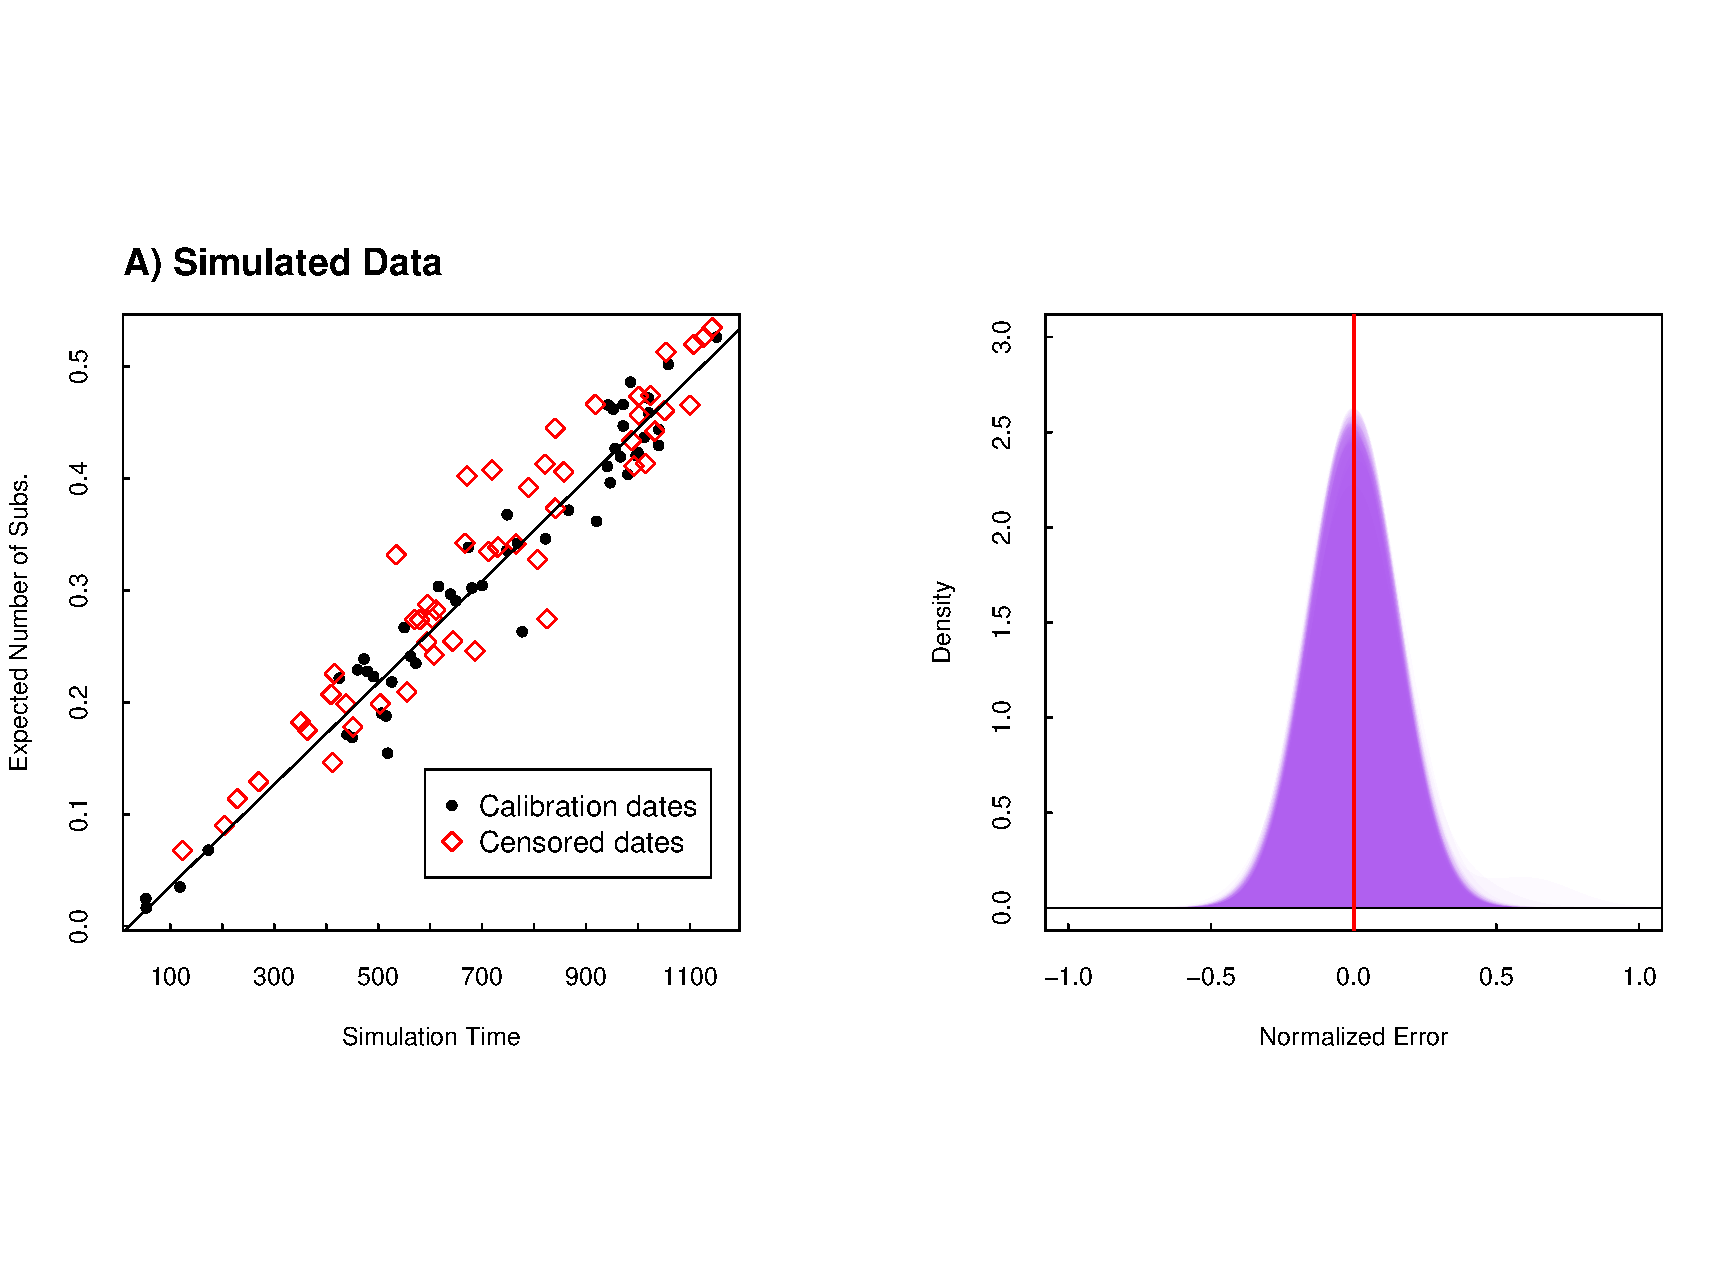
\includegraphics[trim=0cm 0cm 0cm 6cm, clip=true, scale=0.25]{figures/simulated.pdf} \\
	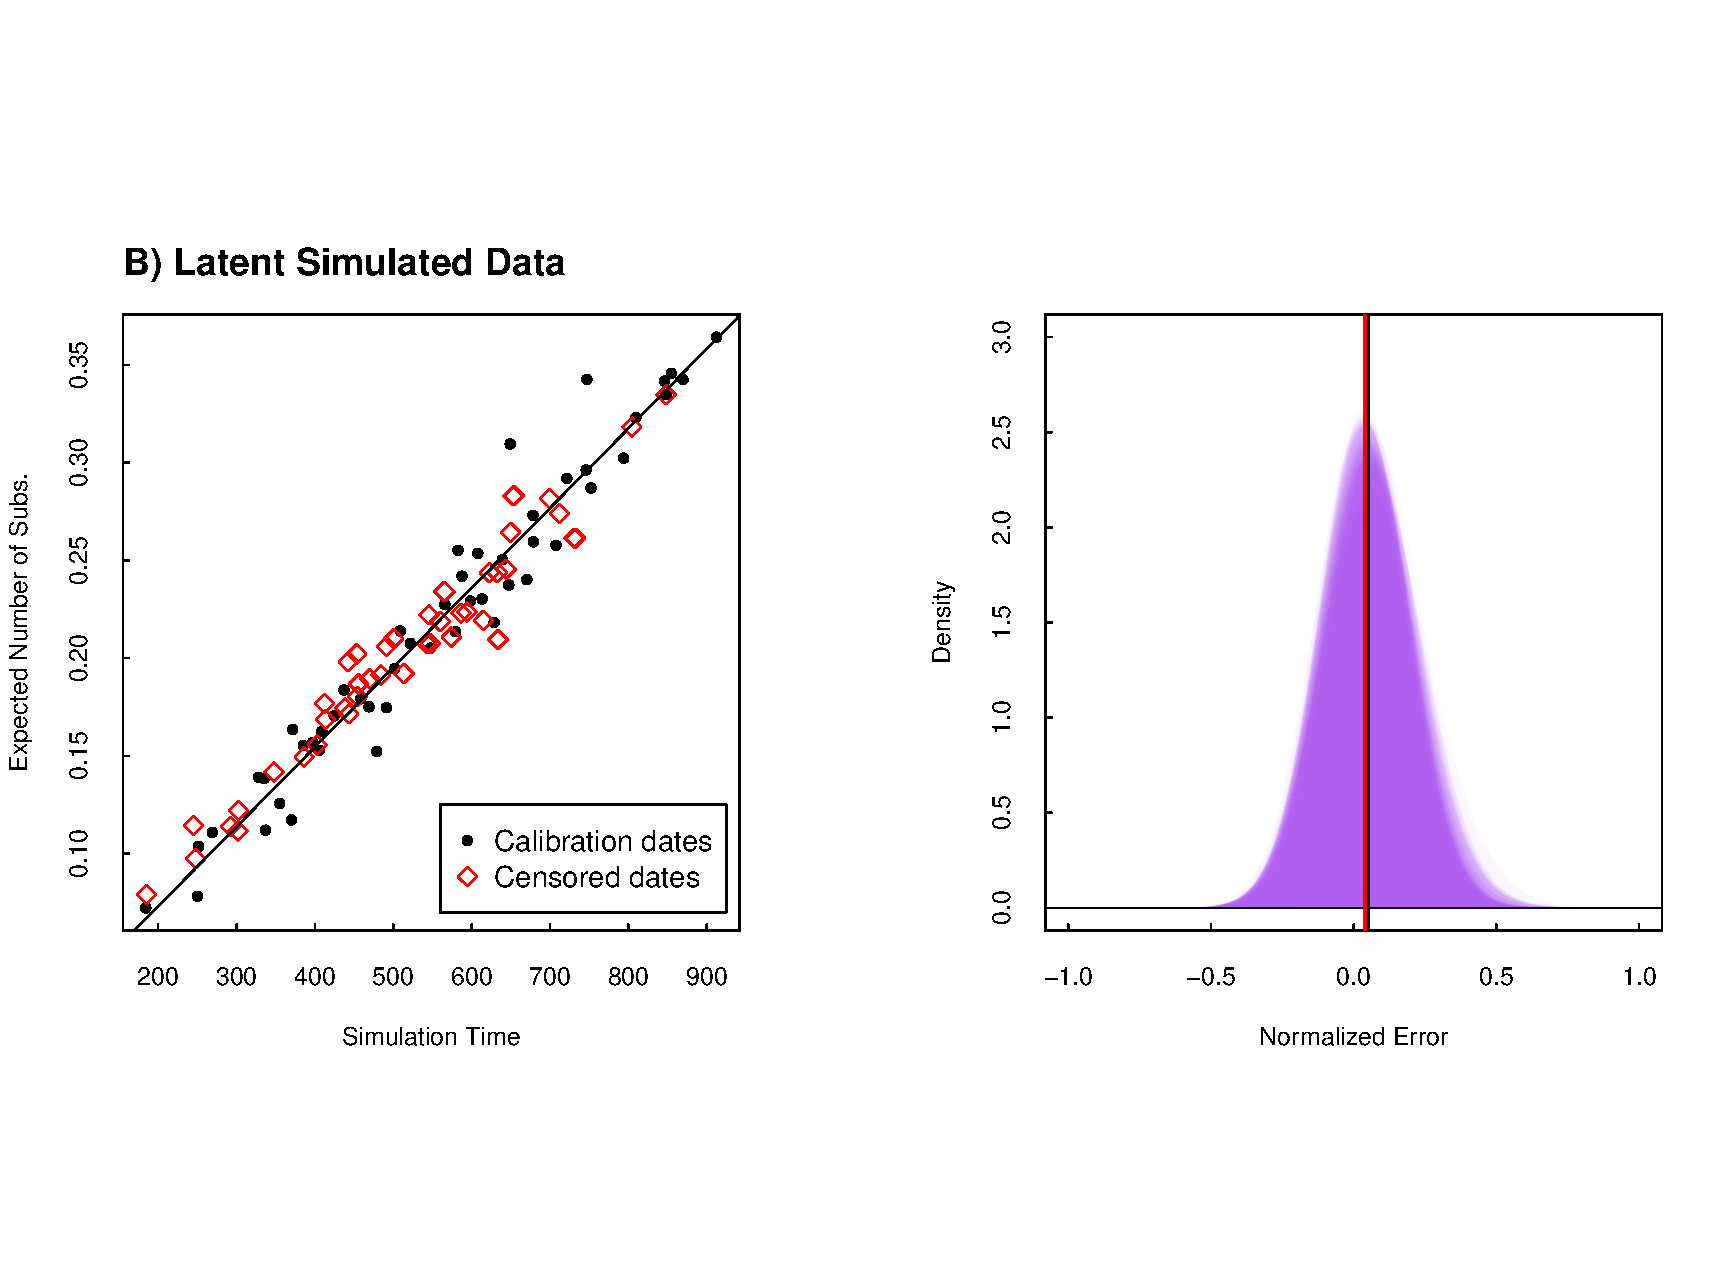
\includegraphics[trim=0cm 0cm 0cm 7cm, clip=true,scale=0.25]{figures/simulated_latent.pdf}\\
	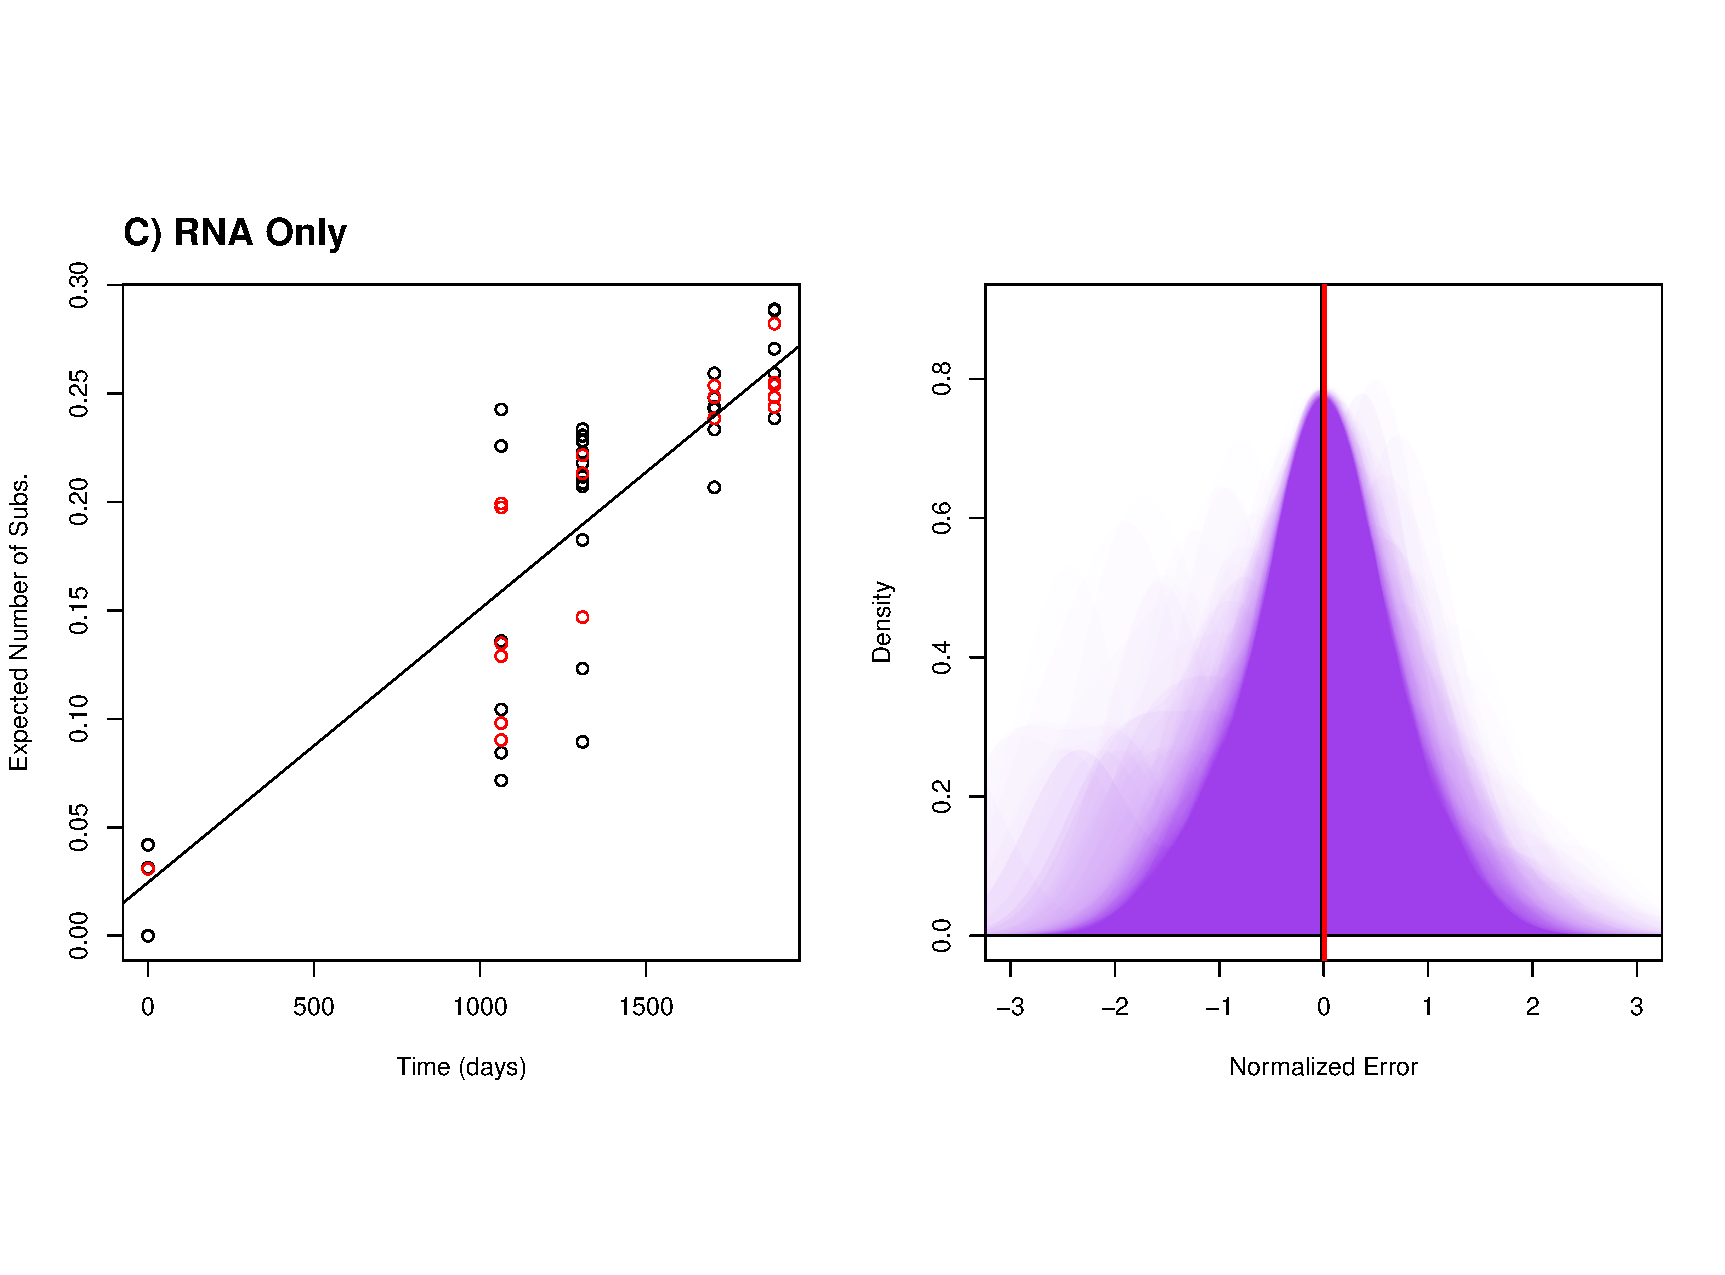
\includegraphics[trim=0cm 0cm 0cm 7cm, clip=true,scale=0.25]{figures/ancre.pdf}\\
	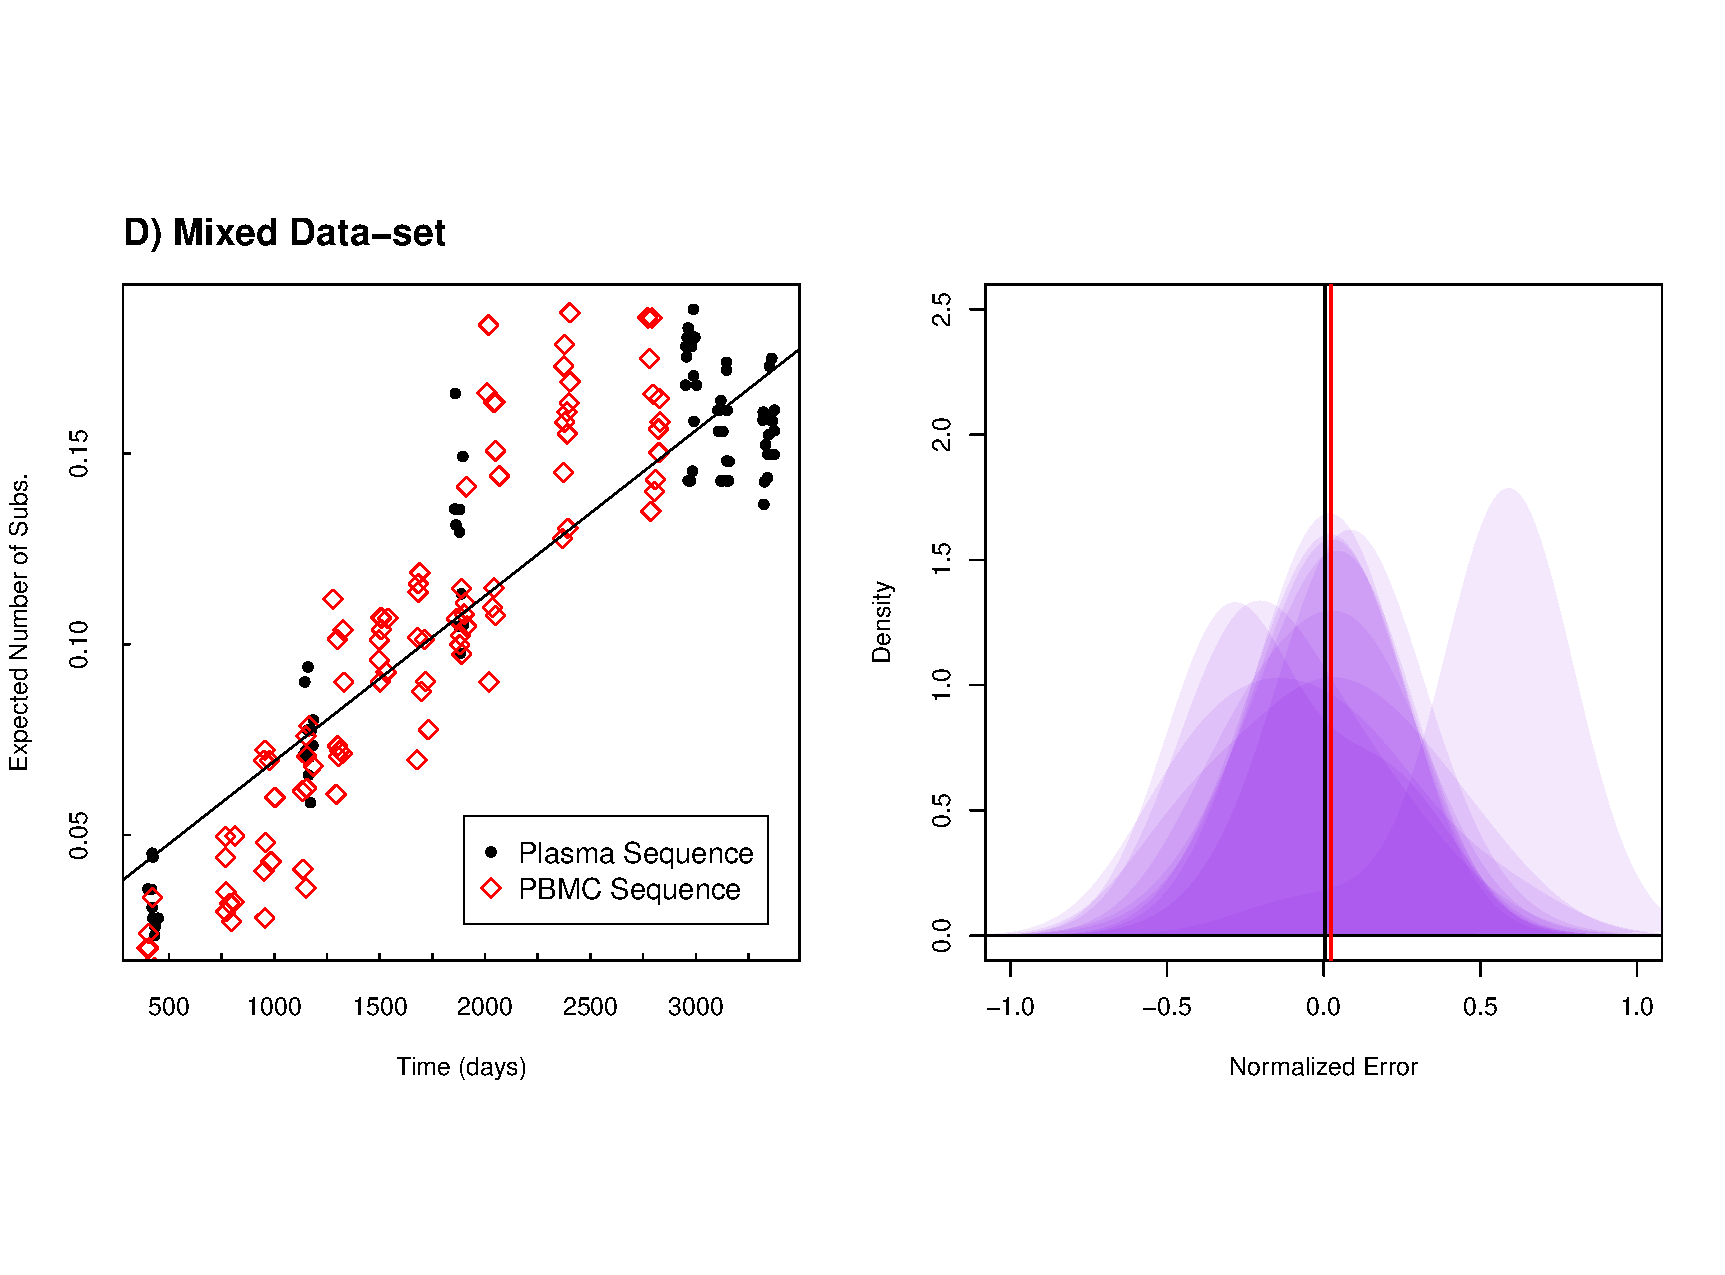
\includegraphics[trim=0cm 4cm 0cm 7cm, clip=true,scale=0.25]{figures/lanl.pdf}
	\caption[Examples]{\anote{Add legend, change points, change shading, explain point colouring, explain mean and median lines.}}
\end{figure}


\subsection{Simulated Data} \label{sec:sim_results}
Very little error in the reconstructed dates,  Simulated data was heavily peaked around 0, little deviation in the histogram. 

\subsection{Simulated Latent Data} \label{sec:sim_lat_results}
Shift of peak.


\subsection{RNA Only Data} \label{sec:rna_only}
Similar to the simulated data, but over a larger range, because genetic variation.

\subsection{Patient Reconstruction}
Qualitatively many plots show examples of latency, qantitavely it's difficult to say. 

